\documentclass[11pt]{article}
\usepackage[margin=1in]{geometry}
\usepackage{booktabs}
\usepackage{graphicx}
\usepackage{float}
\usepackage{caption}
\usepackage{hyperref}
\usepackage[numbers,sort&compress]{natbib}  % Sage Vancouver: numbered
\usepackage{amsmath}
\usepackage{array}

\captionsetup{font=small,labelfont=bf}
\graphicspath{{../05_Figures/}{../08_Model/}}
\makeatletter
\def\input@path{{../06_Tables/}{../08_Model/}}
\makeatother

\title{A Bayesian Left-Censored Joint Longitudinal--Interval Model for
Irregular Molecular Monitoring in Chronic Myeloid Leukemia}

%% ---- TITLE PAGE INFORMATION (submit as a separate, non-anonymized file) ----
%% Xulin Pan (corresponding author), xxp5066@psu.edu
%%   Pennsylvania State University, University Park, PA 16802, USA
%% Jun Lv, School of Mathematics and Statistics, Yunnan University, Kunming, China
%% Chuanming Wang, School of Biological and Food Engineering, Honghe University, Mengzi, China
%% Xueren Wang, School of Mathematics and Statistics, Yunnan University, Kunming, China
%% ---------------------------------------------------------------------------
\author{}     % anonymized for double-anonymized peer review
\date{}

\graphicspath{{../05_Figures/}{../08_Model/}}
\def\input@path{{../06_Tables/}{../08_Model/}}
\renewcommand{\thesection}{S\arabic{section}}
\renewcommand{\thetable}{S\arabic{table}}
\renewcommand{\thefigure}{S\arabic{figure}}

\title{Supplementary Material\\[2pt]
\large A Bayesian Left-Censored Joint Longitudinal--Interval Model for
Irregular Molecular Monitoring in Chronic Myeloid Leukemia}
\author{}
\date{}

\begin{document}
\maketitle

\noindent This supplement collects extensions outlined as future work in the
main paper: a multi-state latent threshold-crossing formulation (onset,
durable response, and molecular relapse), an exploratory informative
visit-process model, a simulation recovery study for the multi-state
estimator, and its application to the CML cohort, together with the secondary
simulation scenarios on endpoint choice and informative monitoring. These
analyses are provided for completeness; the primary analysis in the main paper
is the Bayesian left-censored joint longitudinal--interval model for first
documented DMR.

\bigskip
\section{Proposed model: multi-state latent threshold-crossing (onset, durable response, relapse)}
\label{sec:multistate}

The formulation of Section~3.6 of the main paper defines a single, absorbing
onset. Molecular response, however, has depth and is reversible: a patient may
attain DMR, sustain it, or lose it (molecular relapse), and treatment-free
remission eligibility depends on \emph{durable} MR4.5. These are precisely the
transitions that govern outcome: early and deep response, sustained response,
and loss of response are established predictors of progression-free and overall
survival, and loss of response is itself a clinical event
\cite{Li2014TKIEfficacy,Hanfstein2012EMR}. We therefore extend the
model to a bidirectional multi-state process on the same latent trajectory.
With curvature $\beta_2>0$ the trajectory is convex in $\ell(t)$, so it declines
then rebounds; we define states $0$ (not yet DMR), $1$ (in DMR) and $2$
(molecular relapse), with transitions governed by threshold crossings of
$m_i$. Onset ($0\to1$) is the downward crossing already represented through the
running minimum $M_i(t)=\min_{u\le t}m_i(u)$. \emph{Durable} response over a
window $w$ is the event $\max_{u\in[T_i^D,\,T_i^D+w]} m_i(u)\le c_D$, i.e.\ the
running \emph{maximum} after onset stays below threshold. Relapse ($1\to2$) is
the first upward crossing $T_i^{R}=\inf\{t>T_i^D:m_i(t)>c_D\}$.

Because $m_i$ is quadratic in $\ell$, both extrema are available in closed form:
the running minimum equals the value at the vertex
$\ell^{\ast}=-(\beta_1+b_{1i})/(2\beta_2)$ clamped to $[0,\ell(t)]$, and past the
vertex $m_i$ is monotone increasing, so the upward crossing and the durability
maximum are point evaluations. This removes the soft-min grid approximation
entirely and yields a smooth log density, which in practice eliminates the
divergent transitions induced by the grid.

Each transition is interval-observed and enters the likelihood through the same
probit threshold-crossing device with width $\sigma_{\mathrm{thr}}$: with $M$
the relevant running extremum, a transition documented in $(L,R]$ contributes
$\Phi\{(M(L)-c_D)/\sigma_{\mathrm{thr}}\}-\Phi\{(M(R)-c_D)/\sigma_{\mathrm{thr}}\}$
and a censored transition the corresponding tail. Here $\sigma_{\mathrm{thr}}$
(threshold ambiguity) is separated from the measurement error $\sigma_y$, so the
two scales are identified rather than confounded. Optionally, between-patient
heterogeneity in relapse propensity is captured by a Gaussian frailty
$\rho_i\sim N(0,\sigma_\rho^2)$ on the relapse threshold; because
$\int\Phi\{(x+\rho)/\sigma_{\mathrm{thr}}\}\,\mathrm{d}N(\rho)=
\Phi\{x/\sqrt{\sigma_{\mathrm{thr}}^2+\sigma_\rho^2}\}$, this is equivalent to a
wider relapse-specific width $\sigma_{\mathrm{rel}}=\sqrt{\sigma_{\mathrm{thr}}^2+\sigma_\rho^2}$ and preserves the closed form.

When individual molecular relapse must be captured, the trajectory itself can
be made flexible while retaining a closed form. Adding a patient-specific slope
change $\zeta_i\sim N(0,\sigma_\zeta^2)$ after a knot $\kappa$,
$m_i(\ell)\mathrel{+}{=}\zeta_i(\ell-\kappa)_+$, makes the trajectory
piecewise-quadratic: the running minimum (onset) and post-knot values (relapse)
remain analytic, while individual patients may rebound after $\kappa$ and thereby
relapse. This linear-spline trajectory is the mechanism that captures molecular
relapse in the cohort (Section~\ref{sec:ms-real}).

The model is implemented in
Stan and evaluated by simulation in Section~\ref{sec:msresults}.



\section{Exploratory extension: an informative visit-process model (not fitted)}
\label{sec:visit}

Monitoring intensity may itself depend on molecular response: a patient
doing well may be seen less often, and more frequent testing yields more
opportunities to document DMR. This dependence is not incidental but written
into the governing guideline, which raises molecular-monitoring frequency when
the BCR-ABL transcript rises \cite{CSH2011CMLGuideline}. To assess sensitivity to informative
visiting, we model the visit intensity jointly with the trajectory,
\[
\lambda_i^V(t)=
\exp\{\delta_0+\delta_1[m_i(t)+4.5]+\delta_2\log(1+t)+u_i\},
\qquad u_i\sim N(0,\sigma_u^2),
\]
so that visit intensity depends on the latent MRD, time, and a
patient-level monitoring random effect $u_i$. For visit times
$v_{i1},\ldots,v_{iM_i}$ in $[E_i,C_i]$ the visit-process likelihood is
\[
L_i^V=
\left\{\prod_{\ell=1}^{M_i}\lambda_i^V(v_{i\ell})\right\}
\exp\left\{-\int_{E_i}^{C_i}\lambda_i^V(s)\,ds\right\},
\]
with the cumulative intensity evaluated by quadrature. Because this
extension adds weakly identified parameters in a cohort of 87 patients, it
is presented as a sensitivity model to be evaluated primarily by
simulation and in larger cohorts.



\section{Multi-state extension: recovery of onset, durability, and relapse}
\label{sec:msresults}

We evaluated the multi-state estimator on data simulated from the model, with a
convex trajectory so that onset, durable response, and relapse are all present
(onset rate $0.50$, relapse among responders $0.26$). Across 12 replicates at
$n=300$ every parameter was recovered with negligible bias
(Table~\ref{tab:ms-recovery}); in particular the threshold width
$\sigma_{\mathrm{thr}}$ was recovered essentially exactly (bias $-0.001$),
confirming that separating threshold ambiguity from measurement error restores
the identifiability that a single-width formulation loses. The model-implied
transition probabilities matched empirical rates for all three transitions
(onset $0.503$ vs $0.502$; durable DMR $0.467$ vs $0.494$; relapse $0.134$ vs
$0.129$). Figure~\ref{fig:multistate} illustrates the bidirectional crossings
and this validation.

\begin{table}[!htbp]
\centering
\caption{Multi-state extension: parameter recovery over 12 simulation replicates at $n=300$. Bias and Monte Carlo standard error (MCse) are on the natural scale; $\beta_{\mathrm{time}}$ and $\beta_{\mathrm{time}^2}$ are the linear and quadratic $\log(1+t)$ coefficients.}
\label{tab:ms-recovery}
\small
\begin{tabular}{lrrrr}
\toprule
Parameter & Truth & Mean & Bias & MCse\\
\midrule
$\beta_0$ & $-2.00$ & $-2.009$ & $-0.009$ & $0.023$\\
$\beta_{\mathrm{time}}$ & $-3.60$ & $-3.615$ & $-0.015$ & $0.028$\\
$\beta_{\mathrm{time}^2}$ & $1.30$ & $1.280$ & $-0.020$ & $0.028$\\
$\sigma_y$ & $0.80$ & $0.780$ & $-0.020$ & $0.016$\\
$\tau_{b0}$ & $0.55$ & $0.553$ & $0.003$ & $0.015$\\
$\tau_{b1}$ & $0.75$ & $0.757$ & $0.007$ & $0.012$\\
$\sigma_{\mathrm{thr}}$ & $0.15$ & $0.149$ & $-0.001$ & $0.003$\\
\bottomrule
\end{tabular}
\end{table}

\begin{figure}[!htbp]
\centering
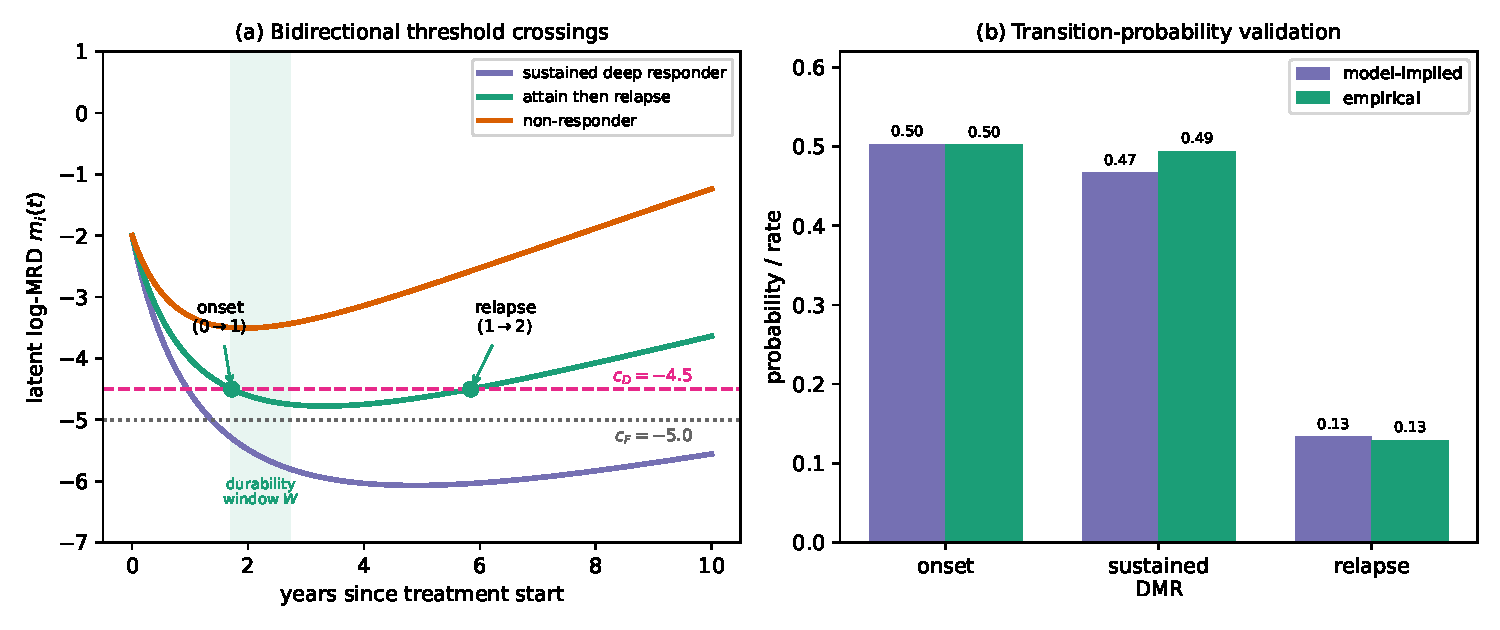
\includegraphics[width=0.98\linewidth]{figure_17_multistate.pdf}
\caption{Bidirectional multi-state threshold model. (a) Example latent log-MRD
trajectories: a sustained deep responder, a patient who attains then relapses
(with onset and relapse crossings of $c_D$ and the durability window $w$
shaded), and a non-responder whose minimum never reaches $c_D$. (b) Model-implied
versus empirical probabilities for the onset, durable-DMR, and relapse
transitions.}
\label{fig:multistate}
\end{figure}



\section{Application of the multi-state model to the CML cohort}
\label{sec:ms-real}

We fitted the multi-state model to the 87-patient cohort
(Table~\ref{tab:ms-real}). Documented transitions comprised 68 DMR onsets
($78\%$) and, under a confirmed definition requiring two consecutive
measurements above $c_D$, 9 molecular relapses ($13\%$ of responders); a raw
definition counting any single post-onset measurement above $c_D$ yielded 30
apparent relapses ($44\%$), most of which are single-visit assay fluctuations
rather than true relapse. The longitudinal estimates reproduce the single-state
fit ($\sigma_y=1.84$, $\beta_{\mathrm{time}}=-3.62$,
$\beta_{\mathrm{time}^2}=0.46$), and the threshold width was cleanly identified
at $\sigma_{\mathrm{thr}}=0.18$ and stable across relapse definitions
($0.17$--$0.18$) --- in contrast to the single-state model, in which this
parameter was not identified. The raw definition, by contrast, distorted the
trajectory (steeper decline and curvature; Table~\ref{tab:ms-real}), confirming
that relapse should be defined on confirmed measurements. Onset was reasonably
calibrated (mean predicted $0.66$ versus observed $0.78$; Brier $0.087$), but
confirmed relapse was under-predicted ($0.02$ versus $0.10$): the
convex-quadratic trajectory rebounds only modestly within follow-up, so it
cannot fully reproduce molecular relapse. We assessed the optional relapse frailty ($\sigma_\rho$): it modestly improved
relapse calibration but was only weakly identified, both here (9 relapses) and
in simulations where the trajectory curvature already explains relapse, so it
yielded little gain over the base model. The dominant limitation is therefore
the trajectory shape rather than relapse heterogeneity. Fitting the
linear-spline trajectory (Section~\ref{sec:multistate}; a patient-specific slope
change after a two-year knot) resolved the under-prediction: the negative
log-likelihood fell by $253$ for one additional variance parameter
($\sigma_\zeta$), and relapse calibration improved markedly (mean predicted
$0.15$ versus observed $0.10$; Brier score $0.082\to0.054$), while the trajectory
remained piecewise-quadratic and hence divergence-free. Full Hamiltonian Monte
Carlo inference for the spline model confirmed these findings and converged
cleanly (all $\widehat R\le1.002$, bulk effective sample size $>2000$): the
rebound heterogeneity was strongly identified ($\sigma_\zeta=6.4$, 90\% interval
$5.0$--$8.0$), and with the flexible trajectory explaining the crossings the
threshold width was near zero ($\sigma_{\mathrm{thr}}=0.06$). These estimates are marginal posterior modes with asymptotic
intervals; the Stan implementation and cohort data are provided for full
Hamiltonian Monte Carlo inference.

\begin{table}[!htbp]
\centering
\caption{Multi-state model fitted to the CML cohort ($N=87$; confirmed-relapse specification). Estimates are marginal posterior modes under the model priors with asymptotic $95\%$ intervals; the final column defines relapse from any single post-onset measurement above $c_D$ (raw). Full posterior intervals should be obtained from the provided Stan data.}
\label{tab:ms-real}
\small
\begin{tabular}{lrrr}
\toprule
Parameter & Estimate & $95\%$ interval & Raw-relapse\\
\midrule
$\beta_0$ & $-1.77$ & $(-1.85,-1.69)$ & $-1.93$\\
$\beta_{\mathrm{time}}$ & $-3.62$ & $(-3.71,-3.54)$ & $-4.22$\\
$\beta_{\mathrm{time}^2}$ & $0.46$ & $(0.33,0.59)$ & $0.77$\\
$\beta_{\mathrm{BM}}$ & $0.73$ & $(0.50,0.96)$ & $0.52$\\
$\sigma_y$ & $1.84$ & $(1.66,2.02)$ & $1.91$\\
$\tau_{b0}$ & $1.05$ & $(1.00,1.11)$ & $1.51$\\
$\tau_{b1}$ & $2.06$ & --- & $2.03$\\
$\sigma_{\mathrm{thr}}$ & $0.18$ & $(0.12,0.24)$ & $0.17$\\
\bottomrule
\end{tabular}
\end{table}


\section{Simulation: endpoint choice and informative monitoring}
\label{sec:s5-sim}

The main-text simulation (Section~6 of the main paper) focuses on the primary
joint model. Here we report the two secondary scenarios summarised in the same
patient-level calibration table (Table~12 of the main paper).

\emph{Endpoint choice.} A latent threshold-crossing estimator, which targets
biological onset rather than the visit-documented endpoint, under-predicted
documented DMR more strongly than the floor model (mean predicted
$\approx0.44$ versus observed $\approx0.85$ at $n=150$; difference
$\approx-0.41$, versus $\approx-0.26$ for the floor model). This quantifies the
distinction between the latent-crossing and documented-DMR estimands: because
documentation occurs only at visits, an estimator that targets biological onset
necessarily predicts fewer \emph{documented} events under interval
ascertainment.

\emph{Informative monitoring.} Under a response-adaptive visit process the
observed documented-DMR rate fell (to $\approx0.59$) and the floor model's
calibration slope rose above one ($1.16$), showing that the monitoring process
materially affects calibration. This motivates the joint visit-process
extension outlined as future work in the main paper, and indicates that under
informative monitoring the conditional-on-schedule analysis should be
complemented by a model for the visit intensity.


\bibliographystyle{unsrtnat}
\bibliography{../07_References/peer_reviewed_papers_selected}

\end{document}
